\chapter{Implementation}

\begin{chapterabstract}
Lorem ipsum dolor sit amet...
\end{chapterabstract}

The following chapter will describe the implementation of the toolkit as envisioned in this thesis, building on the foundation created in the previous analysis and design chapters. 

Implementation focuses primarily on the requirements outlined in Chapter \ref{requirements}, with an emphasis on those of the highest priority. The output of this chapter is the realization of a viable and usable tool.

%______________________________________________________________
\section{Structure of the toolkit}
%______________________________________________________________

The application is designed as a front-end only solution. This architecture simplifies the deployment and dependencies, making it easier to integrate into existing systems. Compared to a full stack solution, it also reduces maintenance and from a security point of view minimizes the attack surface. 

Given it's front-end nature, the configuration's administration can be done through reading from static configuration files rather than relying on data from a backend API. This way, operators of the application can easily adjust the application's behavior and offerings without the need for complex back-end processing, which is not needed in this case as the data are not sensitive or time specific and have a predefined structure. 

Consequently, the toolkit is divided into two main applications: the configurator component and the administrator component. The configurator is the user-facing part that businesses deploy or embed on their webservers, offering the ability to configure products based on the supplied configuration files. The administrator application, on the other hand, is used by the toolkit operators to generate and edit these configuration files.

It should be noted that with this architecture, deploying the administrator application is not a prerequisite for every instance of the configurator; it can be used across various configurators of the same version or even run for the necessary short while in development mode. This flexibility ensures that businesses can manage and update their configurator setups without the need to deploy an instance of the administrator application.

This architecture not only enhances the toolkit's scalability and ease of use, but also ensures that it can be easily integrated into a wide range of business environments, addressing different customization needs without the complexities and overheads associated with traditional back-end-dependent applications.

This structure is also implemented in such a way that if the need for a back-end develops one day, it will be very easy to modify the application for that change.

% - - - - - - - - - - - - - - - - - - - - - - - - - - - - - - -
\subsection{Project directory tree}
% - - - - - - - - - - - - - - - - - - - - - - - - - - - - - - -

\dirtree{%
.1 /.
    .2 apps/.
        .3 admin/.
            .4 src/.
            .4 index.html.
            .4 vite.config.ts.
            .4 package.json.
        .3 main/.
            .4 src/.
            .4 index.html.
            .4 vite.config.ts.
            .4 package.json.
    .2 packages/.
        .3 shared/.
            .4 src/.
            .4 package.json.
    .2 package.json.
}
\vspace{16pt}

Given the separation of the toolkit into the configurator and administrator components, the project is split into two subprojects in the \textquote{apps} directory. The configurator application is located in the main directory, while the admin directory contains the source files for the administrator application. Consequently, each of the subprojects has its own Vite configuration, among their \textquote{index.html} files, \textquote{src} directories for code and \textquote{package.json} for managing the subproject-specific dependencies. 

To minimize code duplication, the \textquote{shared} library is located in the \textquote{packages} directory. This shared library contains common elements imported by both applications, such as data schemes, generic React components, custom React hooks, types and interfaces, CSS styles, or other utility functions. Using this shared package in the configurator and administrator applications ensures consistency and reduces redundancy across the toolkit.

Most dependencies are managed centrally in the root \textquote{package.json} file, with dependencies specific to the subprojects being handled in their corresponding package files. This approach optimizes dependency management across the entire project.

It is important to note that the presented directory tree focuses on illustrating the separation of the project into subprojects: configurator and administrator applications, and the shared library. It is not exhaustive, as the actual project contains various other config and dot files.

The following is a brief overview of the \textquote{src} directories, which organize the source code into logical sections. The directories have the same layout across all subprojects.

\vspace{12pt}
\dirtree{%
.1 src/.
    .2 components/\DTcomment{UI elements, React components}.
    .2 configurations/\DTcomment{configuration of the application}.
    .2 hooks/\DTcomment{custom React hooks}.
    .2 interfaces/\DTcomment{object interfaces}.
    .2 schemas/\DTcomment{data schemas}.
    .2 stores/\DTcomment{data stores and actions}.
    .2 styles/\DTcomment{CSS styles}.
    .2 toasts/\DTcomment{presets for toasts (notifications on top of screen)}.
    .2 utilities/\DTcomment{helper functions and classes}.
}
\vspace{16pt}

\begin{landscape}
\begin{figure}[h]
\centering
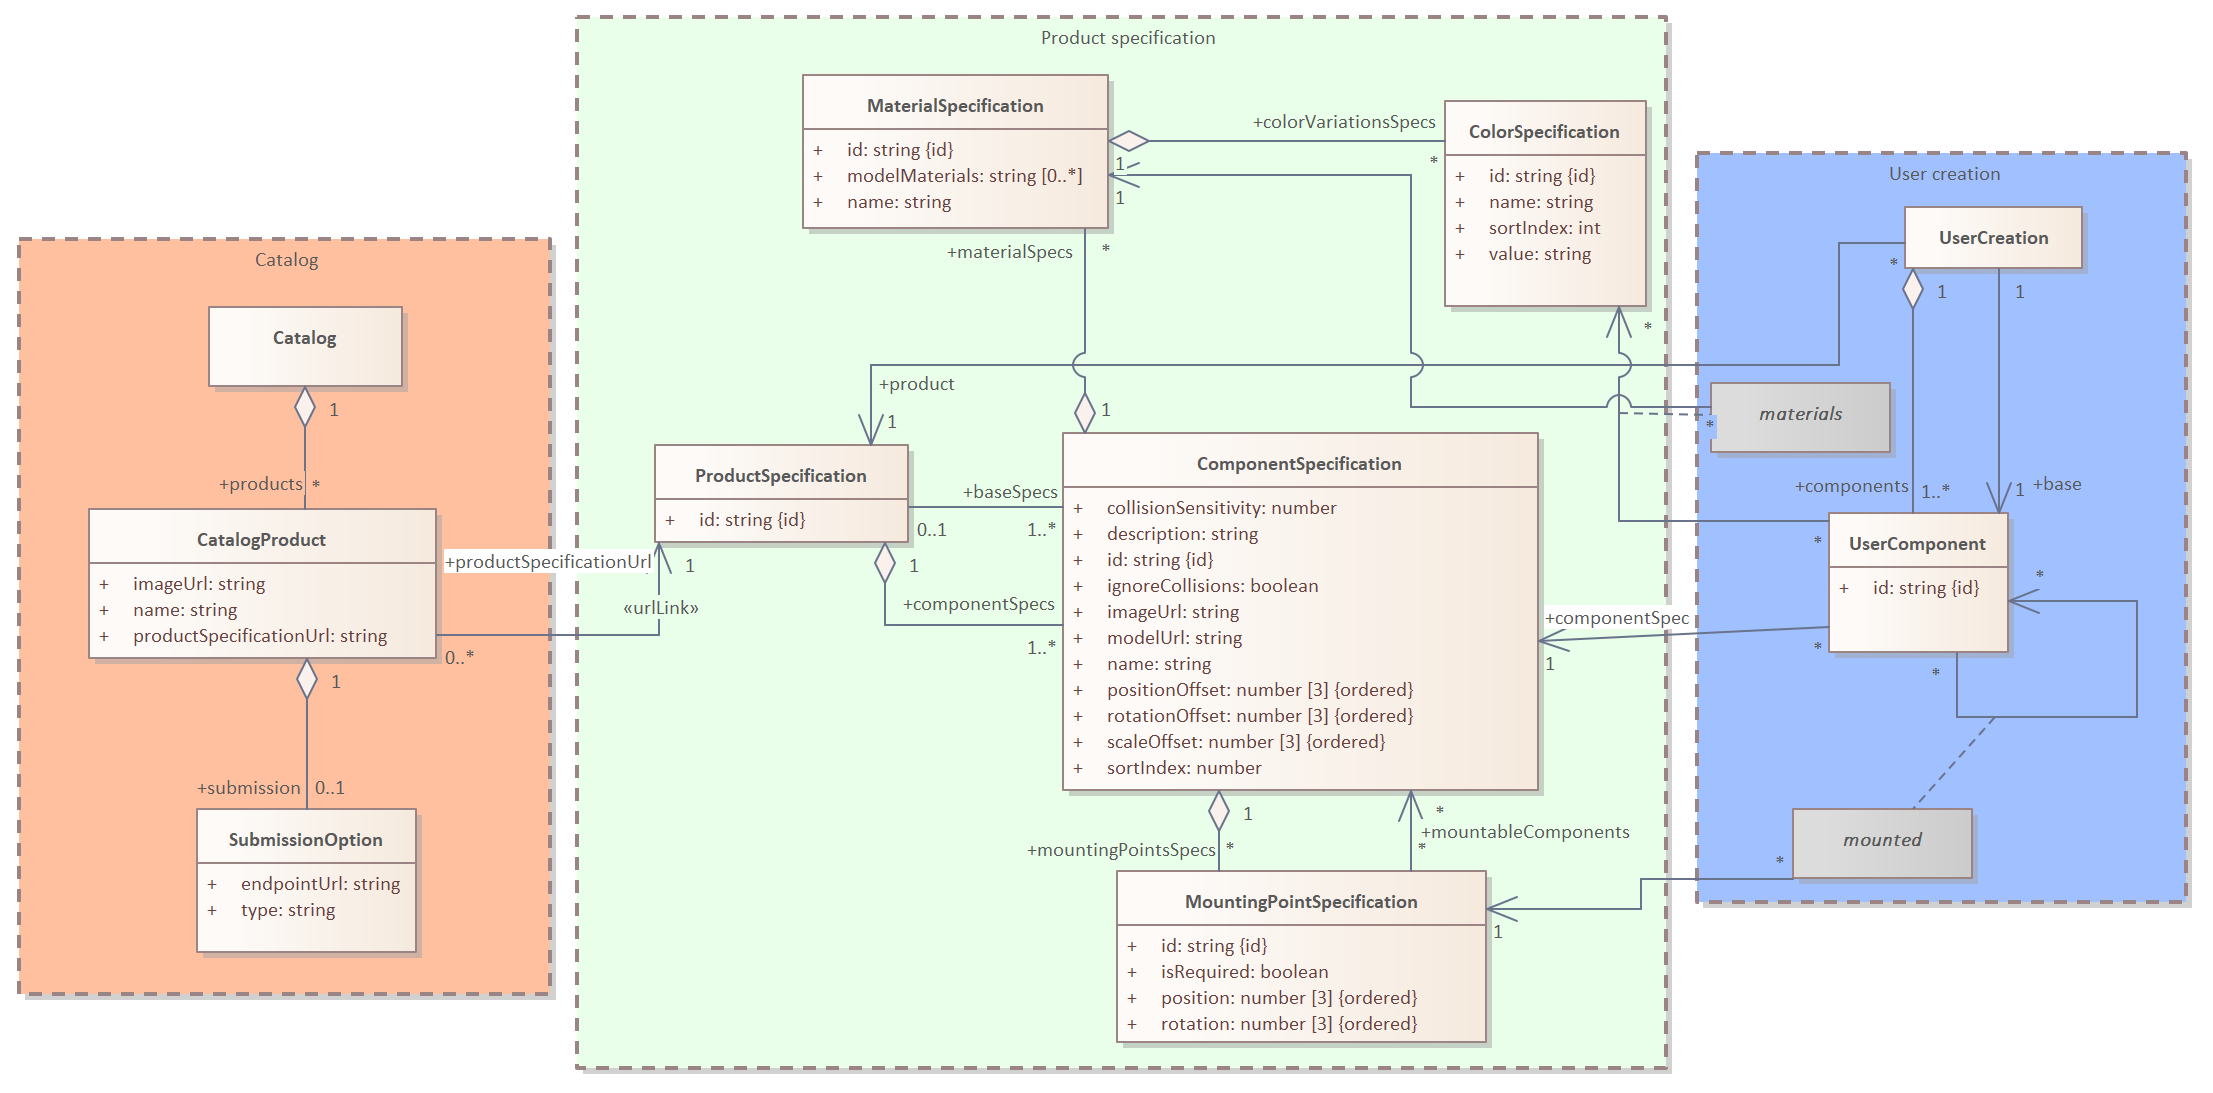
\includegraphics[width=\linewidth]{images/uml_dataschema.png}
\caption{Data schemas as a UML diagram}
\label{fig:data-schema}
\end{figure}
\end{landscape}

\todo{Unimplement baseSpec and prices in code, change size in MaterialSpecification in UML, change color of materials and mounted in UML, rename catalogue to catalog everywhere, add optional attributes in uml, id an product schema}

%______________________________________________________________
\section{Data schemas}
%______________________________________________________________

The data schemas are derived from the domain model discussed in Chapter \ref{domain-model}. These schemas define the shape of the objects that are used to transfer and store information within the tool. 

To visualize these schemas, a UML diagram is provided in Figure \ref{fig:data-schema}. The diagram provides a general overview of utilized the structures and associations, but the implementation requires slight adjustments.

Data schemas are stored in the shared library discussed in the previous section. This ensures consistency, as they are used in both the main and admin applications. 

The schemas are organized into three separate parts: Catalog, product specification, and user creation. Each of these parts corresponds to a separate file in the shared library, in addition to their different roles within the application. The parts are discussed in the following sections, and the UML diagram in Figure \ref{fig:data-schema} provides color coding to differentiate them.

As discussed in Chapter \ref{zod}, the implementation of data schemas utilizes the Zod validation library, which allows straightforward validation of the shape of the data during parsing. TypeScript types are then easily created from these Zod schemas, which is illustrated in Code listing \ref{lst:zod}. \cite{Wycliffe2023} 


% - - - - - - - - - - - - - - - - - - - - - - - - - - - - - - -
\subsection{Catalog}
% - - - - - - - - - - - - - - - - - - - - - - - - - - - - - - -

The catalog data schema, visualized with an orange tint in the UML diagram, is essential for the initial user interaction with the application.

\begin{lstlisting}[caption={~Catalogue schema},label={lst:schema-catalogue},captionpos=b,abovecaptionskip=\medskipamount,belowcaptionskip=\medskipamount]
export const SubmissionOptionSchema = z.object({
  type: SubmissionTypeSchema,
  endpointUrl: z.string().url(),
});

export const CatalogueProductSchema = z.object({
  name: z.string().max(100),
  productSpecificationUrl: z.string(),
  imageUrl: z.string(),
  submission: SubmissionOptionSchema.optional(),
});

export const CatalogueSchema = z.object({
  products: z.record(CatalogueProductSchema),
});
\end{lstlisting}

Building upon the domain model, the catalog is created by the operator of the tool and covers all product specifications. However, compared to the domain model, there is an additional level of abstraction in the form of \textquote{CatalogueProduct}, which contains the most important information about the product specification, such as the name and the preview image. The catalog is separated from the product specifications, which are stored elsewhere. One reason for this is that the catalog will first be fetched when the configuration application is launched, and this information must be presented to the user as soon as possible. The specification of the product, which contains the information needed for the configuration process, can then be fetched from an URL stored inside this object after the user decides which product to configure, which is represented by the stereotype \textquote{urlLink} in the UML diagram.

In addition, each product stores information about the confirmation action in the form of a \textquote{SubmissionOption}, which specifies the type of action and the endpoint to which the application potentially sends the confirmed configuration.

The TypeScript implementation can be seen in Code listing \ref{lst:schema-catalogue}. In the catalogue, each product is stored using a record structure, with ID of the product as a key. The names have been arbitrarily limited to 100 characters to ensure that they can fit within the correct user interface position. URLs, except for the endpoint, are not validated to accommodate local addresses.


% - - - - - - - - - - - - - - - - - - - - - - - - - - - - - - -
\subsection{Product specification}
% - - - - - - - - - - - - - - - - - - - - - - - - - - - - - - -

The advantage of the structure where the catalog is separate from the specifications, which are fetched only when needed, is that each specification can be sourced from a different location. The specifications can also be updated independently on the rest of the catalog.

The product specification part is visualized by a green tint in the UML diagram.  

\begin{lstlisting}[caption={~Product and component specification schema},label={lst:schema-componentspecification},captionpos=b,abovecaptionskip=\medskipamount,belowcaptionskip=\medskipamount]
export const ComponentSpecificationSchema = z.object({
  name: z.string().max(100),
  description: z.string(),
  imageUrl: z.string(),
  modelUrl: z.string(),
  materialSpecs: z.record(MaterialSpecificationSchema),
  mountingPointsSpecs: z.record(MountingPointSpecificationSchema),
  positionOffset: z.tuple(
    [z.number(), z.number(), z.number()]).optional(),
  rotationOffset: z.tuple(
    [z.number(), z.number(), z.number()]).optional(),
  scaleOffset: z.tuple([z.number(), z.number(), z.number()]).optional(),
  ignoreCollisions: z.boolean().optional(),
});

export const BaseSpecificationSchema = z.object({
  component: z.string(),
});

export const ProductSpecificationSchema = z.object({
  baseSpecs: z.record(BaseSpecificationSchema),
  componentSpecs: z.record(ComponentSpecificationSchema),
});
\end{lstlisting}

This part of the data is created by the tool's operator and provides information about the available options for user configuration of a chosen product.

The schemas are also derived from the domain model, although with some modifications such as changes in attributes and some objects being merged.

Most of the concepts in this part are identical to the domain model; however, the new concept of \textquote{base} component is introduced here. Due to the modularity principle, each component is in some way mounted on another component. Base components are such components that can initiate the configuration as they are not mounted to other components. They represent the potentially first component of a configuration. These base components are defined in the product specification.

In the data schema, the model is directly included in the component specification, with the \textquote{modelUrl} attribute pointing to a location with the 3D model file. To compensate for this coupling, attributes that modify the position, rotation, and scale of the model are added to the component specification. Further attributes are also present, such as a description or the option to ignore collisions for this component. The material specification includes the names of the model's meshes in the attribute \textquote{modelMaterials}, and the color specification features the \textquote{sortIndex} attribute, which determines the presentation order to the user.

In TypeScript, the aggregations depicted in the UML diagram are implemented as records, with the IDs serving as keys and the objects as values. Other associations are implemented using solely IDs. Color values are represented using hex code. The implementation of the product and component specifications can be viewed in Code listing \ref{lst:schema-componentspecification}. Other entities in this section are implemented similarly and therefore do not require detailed previews within the text of the thesis.


% - - - - - - - - - - - - - - - - - - - - - - - - - - - - - - -
\subsection{User creation}
% - - - - - - - - - - - - - - - - - - - - - - - - - - - - - - -

User creation corresponds to the configuration entity of domain model, but has been renamed in implementation, as \textquote{configuraiton} is an ambiguous term that can mean several things in application development, for example configuration of the application itself. This makes it clearer what this data schema is representing.

User creation is tinted blue in the UML diagram.

\begin{lstlisting}[caption={~User creation schema},label={lst:schema-usercreation},captionpos=b,abovecaptionskip=\medskipamount,belowcaptionskip=\medskipamount]
export const UserComponentSchema = z.object({
  componentSpec: z.string(),
  materials: z.record(z.string()),
  mounted: z.record(z.string()),
});

export const UserCreationSchema = z.object({
  base: z.string(),
  components: z.record(UserComponentSchema),
});
\end{lstlisting}

User creation stores the configured components, as well as the selected base component, which is the first component of the configuration. All other components are mounted on this component or other components.

In contrast to the domain model, the configured component is represented by \textquote{UserComponent}. This configured component links to a component specification that serves as a template. It also stores information about the mounted components, including the specific mounting points where each component is attached, as well as the selected colors of the materials that have been customized.

In the TypeScript implementation, which can be viewed in the Code listing \ref{lst:schema-usercreation}, the user components are stored in a record with their unique ID as the key. The component specification for each user component is linked by its ID. Information about mounted components are stored in records, with the mounting point specification ID as the key to identify the position and the ID of the user component as the value. Similarly, materials are organized with the material specification ID as the key and the ID of the selected color specification for that material as the value.


%______________________________________________________________
\section{Challenges and solutions}
%______________________________________________________________

\subsection{Component visualization}
\subsubsection{Component interactivity}

\subsection{Model material change}

\subsection{Undo and redo actions}

\subsection{Collision detection}

\subsection{Configuration confirmation}
\subsubsection{Inquiry form}

\subsection{Application configuration}
\subsubsection{Interface texts}

\subsection{Routing}
\subsubsection{Data flow}

\subsection{Catalogue management}

%______________________________________________________________
\section{Views}
%______________________________________________________________